\documentclass[../main.tex]{subfiles}
\graphicspath{{img},{img/ink},{ink}}

\begin{document}

\begin{tcolorbox}[
    width=\textwidth,
    height=\textheight,
    title=Phyphox: Kennlinien von verschiedenen Dioden,
    fonttitle=\Large,
    before title=\vspace{0.2cm}, after title=\vspace{0.2cm},
    colback=white,
    title filled=true, 
    colbacktitle=myorange,
    colframe=black,
    coltitle=black,
    ]

    \vspace{0.2cm}

    \textbf{Klassenstufe}: 9/10

    \vspace{0.5cm}

    \textbf{Fachlicher Bezug}: Kennlinie einer Diode, Anwendungen von Dioden, Mikrocontroller 

    \vspace{0.5cm}
        \textbf{Material}: ESP32 (alternativ: Arduino, Raspberry Pi), Steckbrett + Kabel, Potentiometer, Widerstand $R=220\,\Omega$, LEDs (rot, gelb, grün weiß), normale Diode, Zenerdiode ($2.4$ V), Handy + Phyphox, QR-Code des Experiments

    %\vspace{0.5cm}
    %\textbf{Code}: https://github.com/mx3030/fd2-physik/tree/master/code/Diode
        
    \vspace{0.5cm}
    \begin{minipage}[c]{0.2\textwidth}
        \begin{tikzpicture}
            \ctikzset{
                bipoles/capacitor/width/.initial=.1,
                european resistors
            }
            \coordinate (start) at (0,0);
            \myDAC{start}{red!30}{-0.2cm}{DAC};
        \draw (0.6,0) to [short] (1,0);
        \draw (1,0) to [short] (2,0) coordinate (adc1);
        \myADC{adc1}{white}{0.1cm}{ADC 1};
    \draw (1,0) to [short] (1,-0.3);
    \draw (1,-0.3) to [R={$R$}] (1,-2);
    \draw (1,-2) to [short] (2,-2) coordinate (adc2);
    \myADC{adc2}{orange!30}{0.1cm}{ADC 2};
\draw (1,-2) to [diode] (1,-4);
\draw (1,-4) ++ (0,0.3) node[ground]{}; 
\end{tikzpicture}
\end{minipage}
\hspace{0.5cm}
\begin{minipage}[c]{0.5\textwidth}
    \centering
    \includegraphics[width=1\textwidth]{img/breadboard_qr}
\end{minipage}
\hspace{0.5cm}
\begin{minipage}[c]{0.2\textwidth}
    \centering
    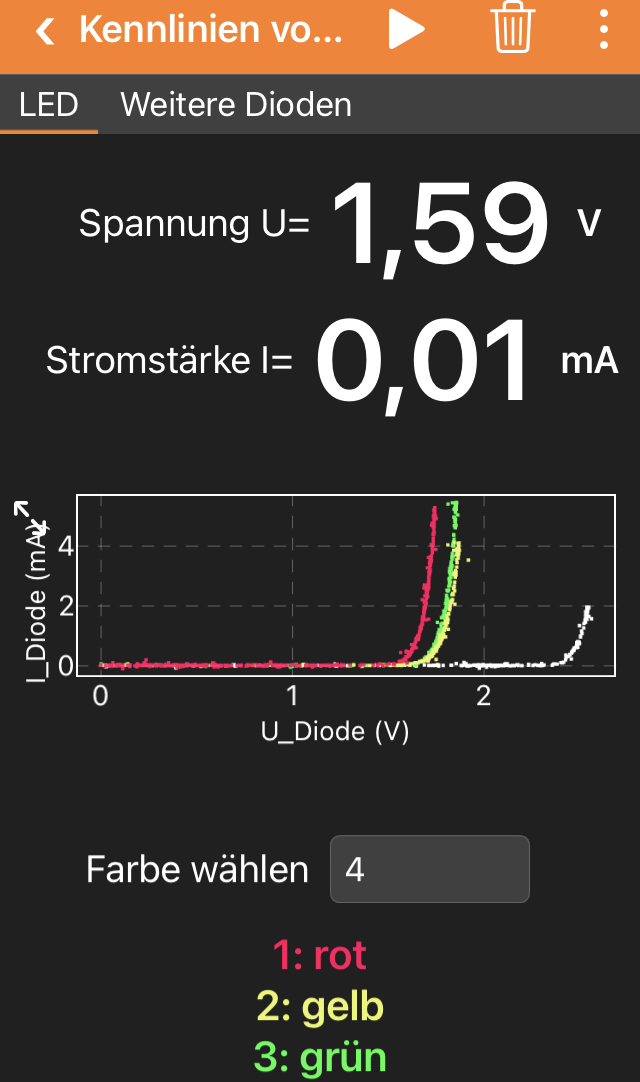
\includegraphics[width=1\textwidth]{img/screen}
\end{minipage}

\vspace{0.5cm}
\begin{minipage}[c]{0.75\textwidth}
    \textbf{Aufbau}: Wird der Versuch als Schülerexperiment durchgeführt, bietet es sich an, Mikrocontroller, Stromversorgung und DAC-Einstellung in einer vorgefertigten Box unterzubringen. Für die weiteren Verbindungen des Schaltkreises können dann vorgefertigte Steckplätze an der Box genutzt werden.\\
In der rechten oberen Ecke der Phyphox-App wird über das + Zeichen das Experiment über einen QR-Code gestartet. 
    \end{minipage}
    \hspace{0.5cm}
    \begin{minipage}[c]{0.2\textwidth}
        \centering
        
\includegraphics[width=1\textwidth]{img/qr_code_phyphox}
    \end{minipage}

    \vspace{0.5cm}
    \textbf{Durchführung}: Während das Experiment läuft (Play-Button gedrückt) wird die Stromstärke gegen den Spannungsabfall über der Diode geplottet. Dabei wird die Farbe verwendet, die im unteren Abschnitt ausgewählt ist. Es werden nacheinander die verschiedenen Dioden eingesetzt und bei jedem Wechsel wird das Experiment kurz pausiert und die entsprechende Farbe eingestellt.

    \vspace{0.5cm}
\textbf{Ergebnis}: Man beobachtet verschiedene Duchbruchspannungen, je nach Farbe der LEDs. 

\vspace{0.5cm}
\textbf{Bemerkungen}: Der DAC eines Mikrocontrollers ermöglicht in der Regel die Einstellung eines Spannungsbereichs von $0-3.3$ V. Da die GPIO-Pins der Mikrokontroller für maximal $3.3$ Volt ausgelegt sind, entstehen hier keine Probleme. Wird eine externe Spannungsquelle verwendet, müssen die ADC-Eingänge zusätzlich vor einer Überschreitung dieser Maximalspannung abgesichert werden. Sollen größere Spannungen gemessen werden, kann im einfachsten Fall ein Spannungsteiler vorgeschaltet werden, der dann in der Software entsprechend berücksichtigt wird.

\end{tcolorbox}


\end{document}
